\documentclass[10pt]{article}
\usepackage{neurips_workshop}

\title{Action-Conditioned Latent World Models\\
for Synthetic Deformable-Object Dynamics}

\author{Anonymous Authors\\
Workshop preprint --- not a real-video or PhysTwin comparison}

\date{}

\begin{document}
% Auto-generated by paper/sync_tables.py — do not edit.
\makeatletter
\newcommand{\NEpisodes}{2000}
\newcommand{\EpisodeLength}{16}
\newcommand{\ImgSize}{64}
\newcommand{\NTransitions}{30{,}000}
\newcommand{\DumpSeed}{0}
\newcommand{\DumpWorkers}{7}
\newcommand{\DumpBackend}{numpy}
\newcommand{\NStiffZero}{667}
\newcommand{\NStiffOne}{667}
\newcommand{\NStiffTwo}{666}
\newcommand{\StiffELow}{18}
\newcommand{\StiffEMid}{70}
\newcommand{\StiffEHigh}{220}
\newcommand{\NTrainPhysics}{1800}
\newcommand{\NValPhysics}{200}
\newcommand{\ChanceStiffness}{0.333}
\newcommand{\ChanceStiffnessPct}{33.3}
\newcommand{\ChanceContact}{0.250}
\newcommand{\ChanceContactPct}{25.0}
\newcommand{\ProbeStiffValMean}{0.339}
\newcommand{\ProbeContactValMean}{0.574}
\newcommand{\ProbeStiffTargetMean}{0.331}
\newcommand{\ProbeStiffTrainMean}{0.350}
\newcommand{\ProbeStiffValRTwo}{-0.002}
\newcommand{\ZTNormStd}{1.1e-04}
\newcommand{\ZTLatentDim}{128}
\newcommand{\ZTDimsBelowGamma}{128}
\newcommand{\ZTHingeBinding}{true}
\newcommand{\BaselineNTrain}{120}
\newcommand{\BaselineNVal}{40}
\newcommand{\BaselineEpochs}{8}
\newcommand{\BaselineDevice}{cpu}
\newcommand{\AblationNVal}{12}
\newcommand{\AblationEpochs}{1}
\newcommand{\AblationDevice}{mps}
\newcommand{\FailureEpisode}{1841}
\newcommand{\FailureMseKten}{0.9651}
\newcommand{\WorkshopMultiseedExists}{false}
\newcommand{\SmokeNVal}{12}
\newcommand{\SmokeNTrain}{36}
\newcommand{\SmokeProbeSE}{0.14}
\newcommand{\WorkshopEpochs}{200}
\newcommand{\PatchSize}{8}
\newcommand{\EmaTau}{0.996}
\newcommand{\VicregSim}{25}
\newcommand{\VicregStd}{25}
\newcommand{\VicregCov}{1}
\newcommand{\VicregGamma}{1}
\newcommand{\EmbedDimYaml}{128}
\newcommand{\ActionDim}{4}
\newcommand{\NStiffClasses}{3}
\newcommand{\NGeometries}{2}
\newcommand{\ShowcaseEpA}{1800}
\newcommand{\ShowcaseEpB}{1801}
\newcommand{\ShowcaseEpC}{1802}
\newcommand{\TrainSeedYaml}{42}
\newcommand{\SeedB}{43}
\newcommand{\NSeeds}{2}
\newcommand{\VicregCompletedEpochs}{133}
\newcommand{\MseCompletedEpochs}{5}
\newcommand{\GitHead}{07167b5}
\newcommand{\TwoSeedExists}{false}
\newcommand{\EffRankTgtVicreg}{NA}
\newcommand{\EffRankDimTgtVicreg}{128}
\newcommand{\EffRankHatVicreg}{NA}
\newcommand{\EffRankDimHatVicreg}{128}
\newcommand{\EffRankTgtMse}{NA}
\newcommand{\EffRankDimTgtMse}{128}
\newcommand{\EffRankHatMse}{NA}
\newcommand{\EffRankDimHatMse}{128}
\newcommand{\TSVicregKOneMean}{NA}
\newcommand{\TSVicregKOneRange}{NA}
\newcommand{\TSVicregKFiveMean}{NA}
\newcommand{\TSVicregKFiveRange}{NA}
\newcommand{\TSVicregKTenMean}{NA}
\newcommand{\TSVicregKTenRange}{NA}
\newcommand{\TSMseKOneMean}{NA}
\newcommand{\TSMseKOneRange}{NA}
\newcommand{\TSMseKFiveMean}{NA}
\newcommand{\TSMseKFiveRange}{NA}
\newcommand{\TSMseKTenMean}{NA}
\newcommand{\TSMseKTenRange}{NA}
\newcommand{\BLVicregKOneMse}{0.145}
\newcommand{\BLVicregKOneStiff}{32.5}
\newcommand{\BLVicregKOneContact}{40.0}
\newcommand{\BLVicregKFiveMse}{0.174}
\newcommand{\BLVicregKFiveStiff}{30.0}
\newcommand{\BLVicregKFiveContact}{22.5}
\newcommand{\BLVicregKTenMse}{0.181}
\newcommand{\BLVicregKTenStiff}{40.0}
\newcommand{\BLVicregKTenContact}{30.0}
\newcommand{\BLNocovKOneMse}{0.247}
\newcommand{\BLNocovKOneStiff}{30.0}
\newcommand{\BLNocovKOneContact}{32.5}
\newcommand{\BLNocovKFiveMse}{0.257}
\newcommand{\BLNocovKFiveStiff}{32.5}
\newcommand{\BLNocovKFiveContact}{20.0}
\newcommand{\BLNocovKTenMse}{0.273}
\newcommand{\BLNocovKTenStiff}{40.0}
\newcommand{\BLNocovKTenContact}{30.0}
\newcommand{\BLMseKOneMse}{5.20e-04}
\newcommand{\BLMseKOneStiff}{40.0}
\newcommand{\BLMseKOneContact}{32.5}
\newcommand{\BLMseKFiveMse}{0.021}
\newcommand{\BLMseKFiveStiff}{40.0}
\newcommand{\BLMseKFiveContact}{35.0}
\newcommand{\BLMseKTenMse}{0.022}
\newcommand{\BLMseKTenStiff}{40.0}
\newcommand{\BLMseKTenContact}{27.5}
\newcommand{\BLPixaeKOneMse}{0.335}
\newcommand{\BLPixaeKOneStiff}{40.0}
\newcommand{\BLPixaeKOneContact}{32.5}
\newcommand{\BLPixaeKFiveMse}{0.325}
\newcommand{\BLPixaeKFiveStiff}{40.0}
\newcommand{\BLPixaeKFiveContact}{35.0}
\newcommand{\BLPixaeKTenMse}{0.326}
\newcommand{\BLPixaeKTenStiff}{40.0}
\newcommand{\BLPixaeKTenContact}{27.5}
\newcommand{\BLNoactKOneMse}{0.239}
\newcommand{\BLNoactKOneStiff}{40.0}
\newcommand{\BLNoactKOneContact}{32.5}
\newcommand{\BLNoactKFiveMse}{0.462}
\newcommand{\BLNoactKFiveStiff}{40.0}
\newcommand{\BLNoactKFiveContact}{35.0}
\newcommand{\BLNoactKTenMse}{0.362}
\newcommand{\BLNoactKTenStiff}{40.0}
\newcommand{\BLNoactKTenContact}{27.5}
\newcommand{\BLGnnKOneMse}{3.32e-08}
\newcommand{\BLGnnKOneStiff}{40.0}
\newcommand{\BLGnnKOneContact}{32.5}
\newcommand{\BLGnnKFiveMse}{8.41e-08}
\newcommand{\BLGnnKFiveStiff}{40.0}
\newcommand{\BLGnnKFiveContact}{35.0}
\newcommand{\BLGnnKTenMse}{9.81e-08}
\newcommand{\BLGnnKTenStiff}{40.0}
\newcommand{\BLGnnKTenContact}{27.5}
\newcommand{\AblFullKOneMse}{0.172}
\newcommand{\AblFullKFiveMse}{0.188}
\newcommand{\AblFullKTenMse}{0.199}
\newcommand{\AblFullKTwentyMse}{0.199}
\newcommand{\AblAKOneMse}{0.286}
\newcommand{\AblAKFiveMse}{0.362}
\newcommand{\AblAKTenMse}{0.494}
\newcommand{\AblAKTwentyMse}{0.338}
\newcommand{\AblBKOneMse}{0.011}
\newcommand{\AblBKFiveMse}{0.063}
\newcommand{\AblBKTenMse}{0.063}
\newcommand{\AblBKTwentyMse}{0.063}
\newcommand{\AblCKOneMse}{0.108}
\newcommand{\AblCKFiveMse}{0.106}
\newcommand{\AblCKTenMse}{0.106}
\newcommand{\AblCKTwentyMse}{0.106}
\makeatother

\maketitle

\begin{abstract}
We study action-conditioned joint-embedding predictive architectures (AC-JEPA) as
latent world models of \emph{synthetic} deformable-object dynamics. Observations
come from an in-repo MLS-MPM renderer (\NEpisodes{} episodes, $T{=}$\EpisodeLength{},
$\ImgSize\times\ImgSize$), not from captured video, and we do not claim results
on PhysWorld or PhysTwin. The contribution is a controlled comparison: VICReg
versus covariance-ablated / MSE-only / pixel-space alternatives, plus an
action-conditioning knockout, against a particle-GNN baseline in the
\emph{same} mass-spring simulator. On a scaled physics dump
($n_{\mathrm{val}}{=}$\NValPhysics{}), contact-quadrant linear probes beat chance
(\ProbeContactValMean{} vs.\ \ChanceContact{}) while stiffness class remains at
chance (\ProbeStiffValMean{} vs.\ \ChanceStiffness{}), including an oracle probe
on the EMA target. We report that limitation rather than a new SOTA number.
Workshop-scale mean\,$\pm$\,std ablations have not been generated.
\end{abstract}

\section{Introduction}
Learned world models that forecast how a deformable object will respond to
contact would be useful for manipulation, but the recent digital-twin literature
is dominated by systems that start from \emph{real video} and an MPM-optimized
twin~\citep{jiang2025phystwin,yang2025physworld}. This paper asks a narrower
question on a fully synthetic stack: if we train an action-conditioned JEPA
\citep{assran2023ijepa,bardes2024vjepa} with VICReg~\citep{bardes2022vicreg} on
rendered MLS-MPM frames~\citep{hu2018mlsmpm}, which pieces of the objective and
which form of action fusion actually matter, and what physical properties are
linearly readable from the latent?

We do \textbf{not} claim to outperform PhysWorld or PhysTwin. Those methods
operate in a different domain (real captures, reconstructed geometry, privileged
particle twins). Our numbers are within-simulator. The empirical payload is
(i)~a six-way baseline on a shared mass-spring split
(Table~\ref{tab:baselines}), (ii)~a dummy-scale loss ablation imported from the
exporter so cells cannot drift from \texttt{outputs/} (Table~\ref{tab:ac-jepa-ablation}),
and (iii)~probe diagnostics on the physics dump that put stiffness non-decodability
on the record (Section~\ref{sec:limitations}).

\section{Related work}
\paragraph{JEPA and VICReg.}
I-JEPA~\citep{assran2023ijepa} and V-JEPA~\citep{bardes2024vjepa} learn by
predicting embeddings of a target view from a context view, with an EMA target
encoder in the BYOL family~\citep{grill2020byol}. AC-JEPA instantiates that
recipe on $(x_t,a_t)\mapsto z_{t+1}$. Collapse is regularized with
VICReg~\citep{bardes2022vicreg}: invariance, a per-dimension variance hinge, and
an off-diagonal covariance penalty, implemented in \texttt{src/losses.py}.

\paragraph{Particle-graph world models.}
DPI-Net~\citep{li2019dpinet} and GNS~\citep{sanchezgonzalez2020gns} propagate
messages on particle graphs to predict the next state. Our particle-GNN baseline
reuses the simulator's spring \texttt{\_edge\_list} and is scored in graph-readout
space; it is a within-simulator relative of that family, not a reimplementation
of those papers' datasets.

\paragraph{Real-video digital twins (domain gap).}
PhysTwin~\citep{jiang2025phystwin} reconstructs and resimulates deformables from
sparse video with a physics-informed twin. PhysWorld~\citep{yang2025physworld}
fits an MPM twin to real video, synthesizes demonstrations, and trains a GNN for
real-time prediction. Both start from captured footage of a small number of
objects. Our dump is synthetic RGB of disks/bars with three global Young's
moduli, no camera, no residual physics mismatch. Table~\ref{tab:baselines} is
therefore not a SOTA table against those systems.

\section{Method}
\paragraph{Architecture.}
Following \texttt{src/models/ac\_jepa.py} and \texttt{ModelConfig}, AC-JEPA has
three modules. An online encoder $f_\theta$ (ViT by default) maps a frame
$x_t$ to $z_t$. An action-conditioned predictor $g_\phi$ maps $(z_t,a_t)$ to
$\hat z_{t+1}$. A target encoder $f_{\bar\theta}$ is an EMA copy
$\bar\theta \leftarrow \tau\bar\theta + (1-\tau)\theta$ with default
$\tau{=}$\EmaTau{}; it produces the stop-gradient target $z_{t+1}=f_{\bar\theta}(x_{t+1})$.
Only $f_\theta$ and $g_\phi$ receive gradients. Workshop YAML uses
$\ImgSize\times\ImgSize$ frames, patch size \PatchSize{}, embedding width
\ZTLatentDim{}, concat fusion, and $a_t\in\mathbb{R}^{\ActionDim{}}$
(contact $xy$ + force $xy$). Setting \texttt{condition\_on\_action=False} drops
$a_t$ so $g_\phi$ sees $z_t$ only (no-action ablation).

\paragraph{Objectives.}
\texttt{prediction\_objective} in \texttt{src/losses.py} implements four latent
losses on $(\hat z_{t+1}, z_{t+1})$: (i)~full VICReg
($\lambda{=}$\VicregSim{}, $\mu{=}$\VicregStd{}, $\nu{=}$\VicregCov{}, $\gamma{=}$\VicregGamma{});
(ii)~Variant~A, \texttt{vicreg\_no\_cov}, invariance + variance only;
(iii)~Variant~B, invariance MSE only;
(iv)~optional smooth-$\ell_1$ / cosine stand-ins for the invariance term.
Variant~C is a pixel-space autoencoder that decodes $g_\phi(z_t,a_t)$ to
$\hat x_{t+1}$ rather than matching $z_{t+1}$. Open-loop evaluation applies the
predictor for $k$ steps without replacing $\hat z$ by the true encoding.

\section{Experiments}
\paragraph{Data.}
Prompt~1 writes \texttt{outputs/physics\_mpm/}: \NEpisodes{} episodes of length
\EpisodeLength{}, $\ImgSize\times\ImgSize$ RGB, backend \texttt{\DumpBackend{}}
MLS-MPM (not a Taichi install), dump seed \DumpSeed{}, geometries disk/bar,
$E\in\{\StiffELow,\StiffEMid,\StiffEHigh\}$ with counts
$\NStiffZero/\NStiffOne/\NStiffTwo$ (\texttt{outputs/dataset\_report.json}).
The workshop split is $n_{\mathrm{train}}{=}$\NTrainPhysics{},
$n_{\mathrm{val}}{=}$\NValPhysics{}. Prompt~4 baselines instead use an
in-process mass-spring lattice
($n_{\mathrm{train}}{=}$\BaselineNTrain{}, $n_{\mathrm{val}}{=}$\BaselineNVal{},
\BaselineEpochs{} epochs, device \texttt{\BaselineDevice{}}).

\paragraph{Within-simulator baselines.}
Table~\ref{tab:baselines} is generated from
\texttt{outputs/baseline\_comparison.csv} (no hand-copied cells). VICReg latent
MSE at $k{=}1,5,10$ is $\BLVicregKOneMse$, $\BLVicregKFiveMse$,
$\BLVicregKTenMse$. Dropping the action
(\texttt{no\_action}) raises $k{=}5$ MSE from $\BLVicregKFiveMse$ to
$\BLNoactKFiveMse$ on this split: the predictor uses $a_t$ when it is available.
MSE-only records a much smaller latent MSE ($\BLMseKOneMse$ at $k{=}1$) --- as
expected when the objective is pure invariance and is free to collapse
directions VICReg would keep alive. The particle GNN's $k{=}1$ MSE
($\BLGnnKOneMse$) is \emph{not} in the same space; we do not rank it against
ViT latents. Stiffness probes on this split sit near chance for every method
(e.g.\ VICReg $\BLVicregKOneStiff$\% vs.\ $\ChanceStiffnessPct$\%).

\begin{table}[t]
  \centering
  \small
  \caption{Within-simulator baseline comparison on the mass-spring lattice ($n_{\mathrm{train}}=120$, $n_{\mathrm{val}}=40$, 8 epochs, device \texttt{cpu}). Open-loop rollout MSE ($\downarrow$) at $k\in\{1,5,10\}$. Linear-probe accuracy ($\uparrow$, \%) at $k{=}1$; chance is 33.3\% stiffness / 25.0\% contact. Particle-GNN \texttt{rollout\_mse} is in pooled graph-readout space, not the ViT latent --- magnitudes are not interchangeable across rows. Source: \texttt{outputs/baseline\_comparison.csv}.}
  \label{tab:baselines}
  \setlength{\tabcolsep}{3.5pt}
  \begin{tabular}{lccccc}
    \toprule
    Method & $k{=}1$ & $k{=}5$ & $k{=}10$ & Stiff.\ \% & Contact \% \\
    \midrule
    AC-JEPA (VICReg) & 0.145 & 0.174 & 0.181 & 32.5 & 40.0 \\
    AC-JEPA (no covariance) & 0.247 & 0.257 & 0.273 & 30.0 & 32.5 \\
    AC-JEPA (MSE-only) & \textbf{5.20e-04} & \textbf{0.021} & \textbf{0.022} & 40.0 & 32.5 \\
    Pixel autoencoder & 0.335 & 0.325 & 0.326 & 40.0 & 32.5 \\
    No action conditioning & 0.239 & 0.462 & 0.362 & 40.0 & 32.5 \\
    Particle GNN (GNS/DPI-Net family) & 3.32e-08 & 8.41e-08 & 9.81e-08 & 40.0 & 32.5 \\
    \bottomrule
  \end{tabular}
\end{table}


\paragraph{Loss ablation (dummy scale, imported).}
Table~\ref{tab:ac-jepa-ablation} is the tabular environment from
\texttt{outputs/paper\_tables.tex} with an honest caption. It is a
\AblationEpochs{}-epoch, $n_{\mathrm{val}}{=}$\AblationNVal{} lattice run on
\texttt{\AblationDevice{}}. Workshop mean\,$\pm$\,std
(\texttt{outputs/ablation\_multiseed.json}) does not exist; we include the
placeholder Table~\ref{tab:ac-jepa-ablation-multiseed} rather than inventing
error bars.

\begin{table}[t]
  \centering
  \small
  \caption{Single-seed dummy-scale ablation imported from \texttt{outputs/paper\_tables.tex} (MSE cells from \texttt{outputs/ablation\_results.csv}; probes/latency from a later live eval of the same checkpoints). $n_{\mathrm{val}}=12$, 1 training epoch, device \texttt{mps}, synthetic lattice --- \textbf{not} the workshop 200-epoch / 3-seed study. Workshop mean\,$\pm$\,std JSON is missing (\texttt{outputs/ablation\_multiseed.json} does not exist). Do not read this table as a scaled result.}
  \label{tab:ac-jepa-ablation}
  \begin{tabular}{lccccccrr}
    \toprule
    & \multicolumn{4}{c}{Rollout MSE $\downarrow$}
      & \multicolumn{2}{c}{Probe acc.\ $\uparrow$ (\%)}
      & \multicolumn{2}{c}{Latency} \\
    \cmidrule(lr){2-5}
    \cmidrule(lr){6-7}
    \cmidrule(lr){8-9}
    Method & $k{=}1$ & $k{=}5$ & $k{=}10$ & $k{=}20$ & Stiffness & Friction & FPS $\uparrow$ & ms/frame $\downarrow$ \\
    \midrule
    Full AC-JEPA (VICReg) & 0.172 & 0.188 & 0.199 & 0.199 & \textbf{37.5} & \textbf{29.2} & 608.5 & 1.64 \\
    Variant A (No Covariance) & 0.286 & 0.362 & 0.494 & 0.338 & 37.5 & \textbf{29.2} & 374.3 & 2.67 \\
    Variant B (MSE-only) & \textbf{0.011} & \textbf{0.063} & \textbf{0.063} & \textbf{0.063} & 35.4 & 22.9 & \textbf{786.8} & \textbf{1.27} \\
    Variant C (Pixel Autoencoder) & 0.108 & 0.106 & 0.106 & 0.106 & \textbf{37.5} & 22.9 & 732.3 & 1.37 \\
    \bottomrule
  \end{tabular}
\end{table}

\begin{table}[t]
  \centering
  \small
  \caption{Workshop-scale multi-seed ablation (mean\,$\pm$\,std over seeds 42/43/44 on the MLS-MPM dump) has \textbf{not been generated}: \texttt{outputs/ablation\_multiseed.json} is absent. See \texttt{MAPPING.md}.}
  \label{tab:ac-jepa-ablation-multiseed}
  \begin{tabular}{l}
    \toprule
    No mean\,$\pm$\,std rows to include. \\
    \bottomrule
  \end{tabular}
\end{table}


\paragraph{Qualitative rollouts.}
Figure~\ref{fig:rollouts} shows held-out MLS-MPM episodes at
$k\in\{1,5,10\}$ for $E\in\{\StiffELow,\StiffEMid,\StiffEHigh\}$. VICReg columns
use a \emph{post-hoc} frozen-latent pixel decoder that is not part of AC-JEPA;
the Pixel-AE row is a short qualitative fit, not a \WorkshopEpochs{}-epoch Variant~C
(\texttt{outputs/figures/README.txt}). Figure~\ref{fig:failure} is validation
episode \FailureEpisode{}, the worst latent MSE at $k{=}10$
(\FailureMseKten{}; $n_{\mathrm{val}}{=}$\NValPhysics{}).

\begin{figure}[t]
  \centering
  \begin{minipage}{0.32\linewidth}
    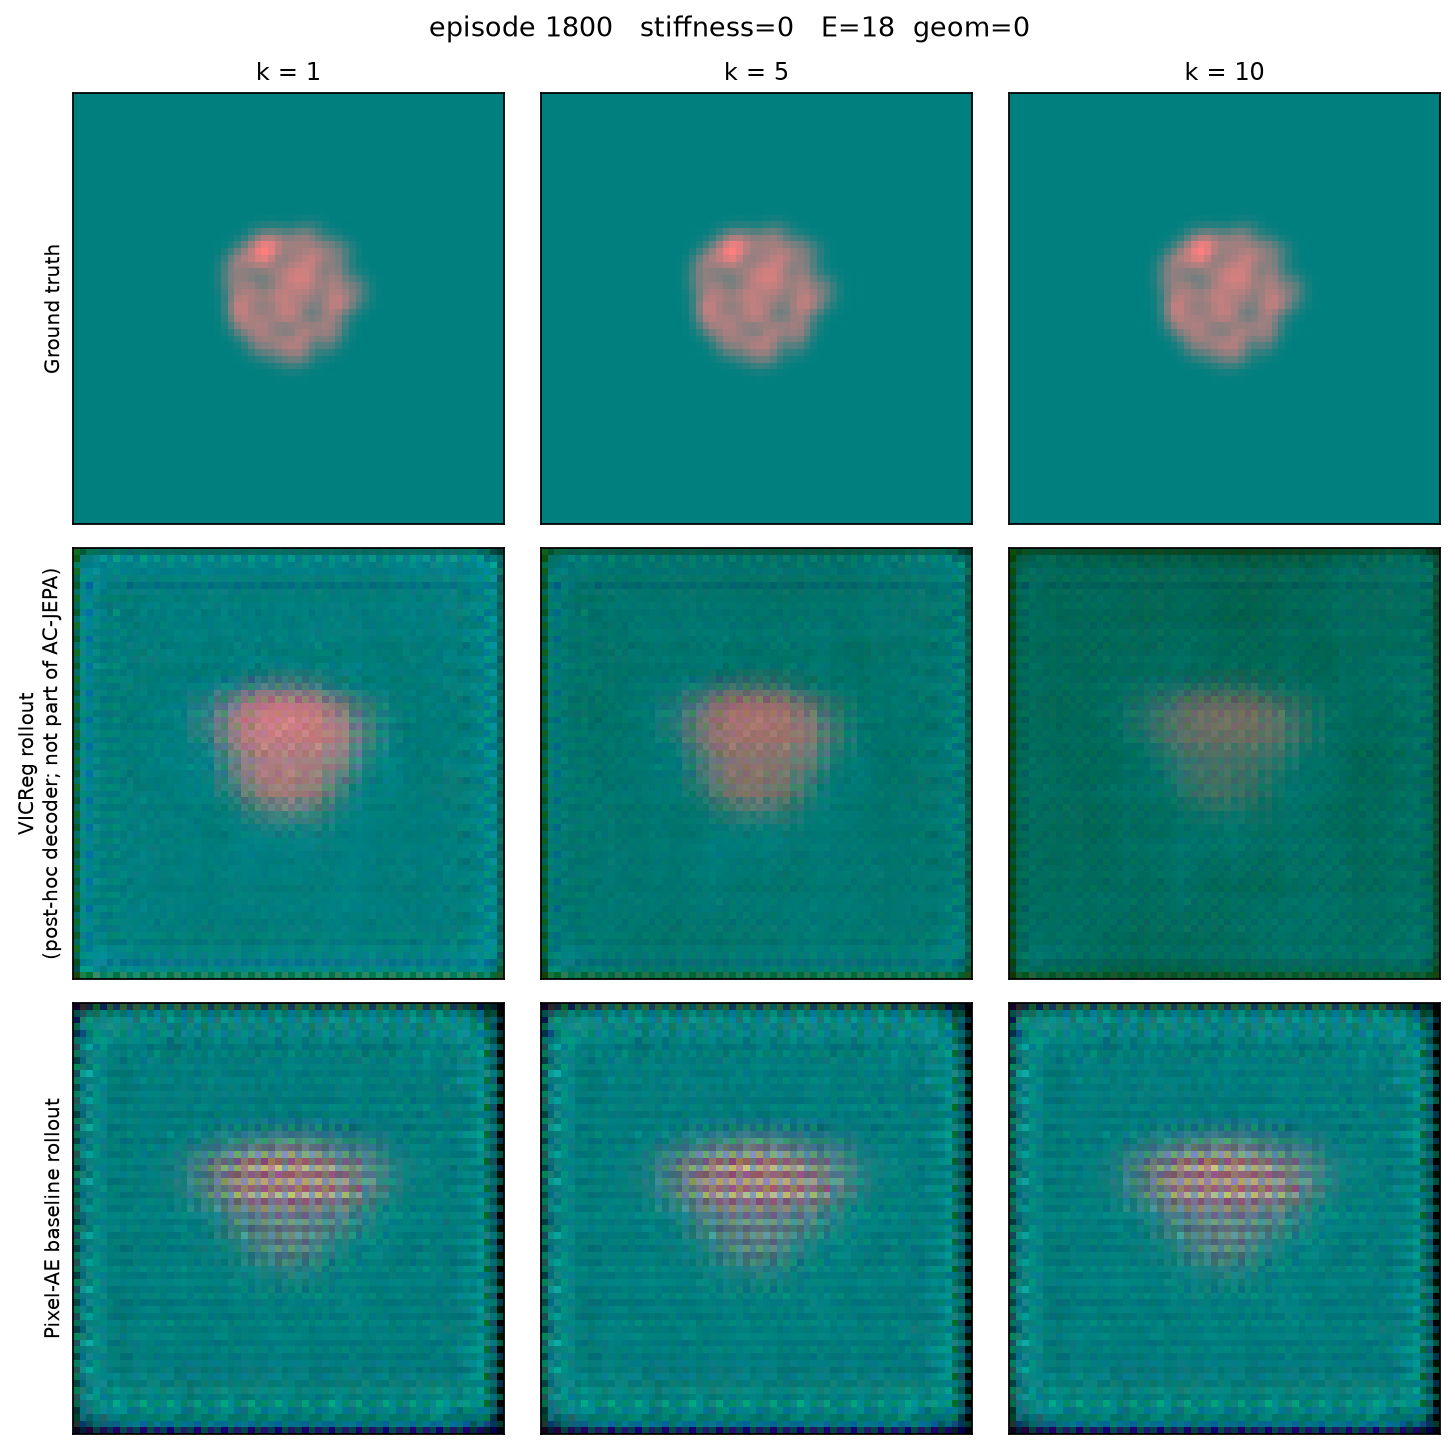
\includegraphics[width=\linewidth]{../outputs/figures/rollout_comparison_1800.png}\\[-2pt]
    {\scriptsize $E{=}\StiffELow$ (ep.\ \ShowcaseEpA{})}
  \end{minipage}\hfill
  \begin{minipage}{0.32\linewidth}
    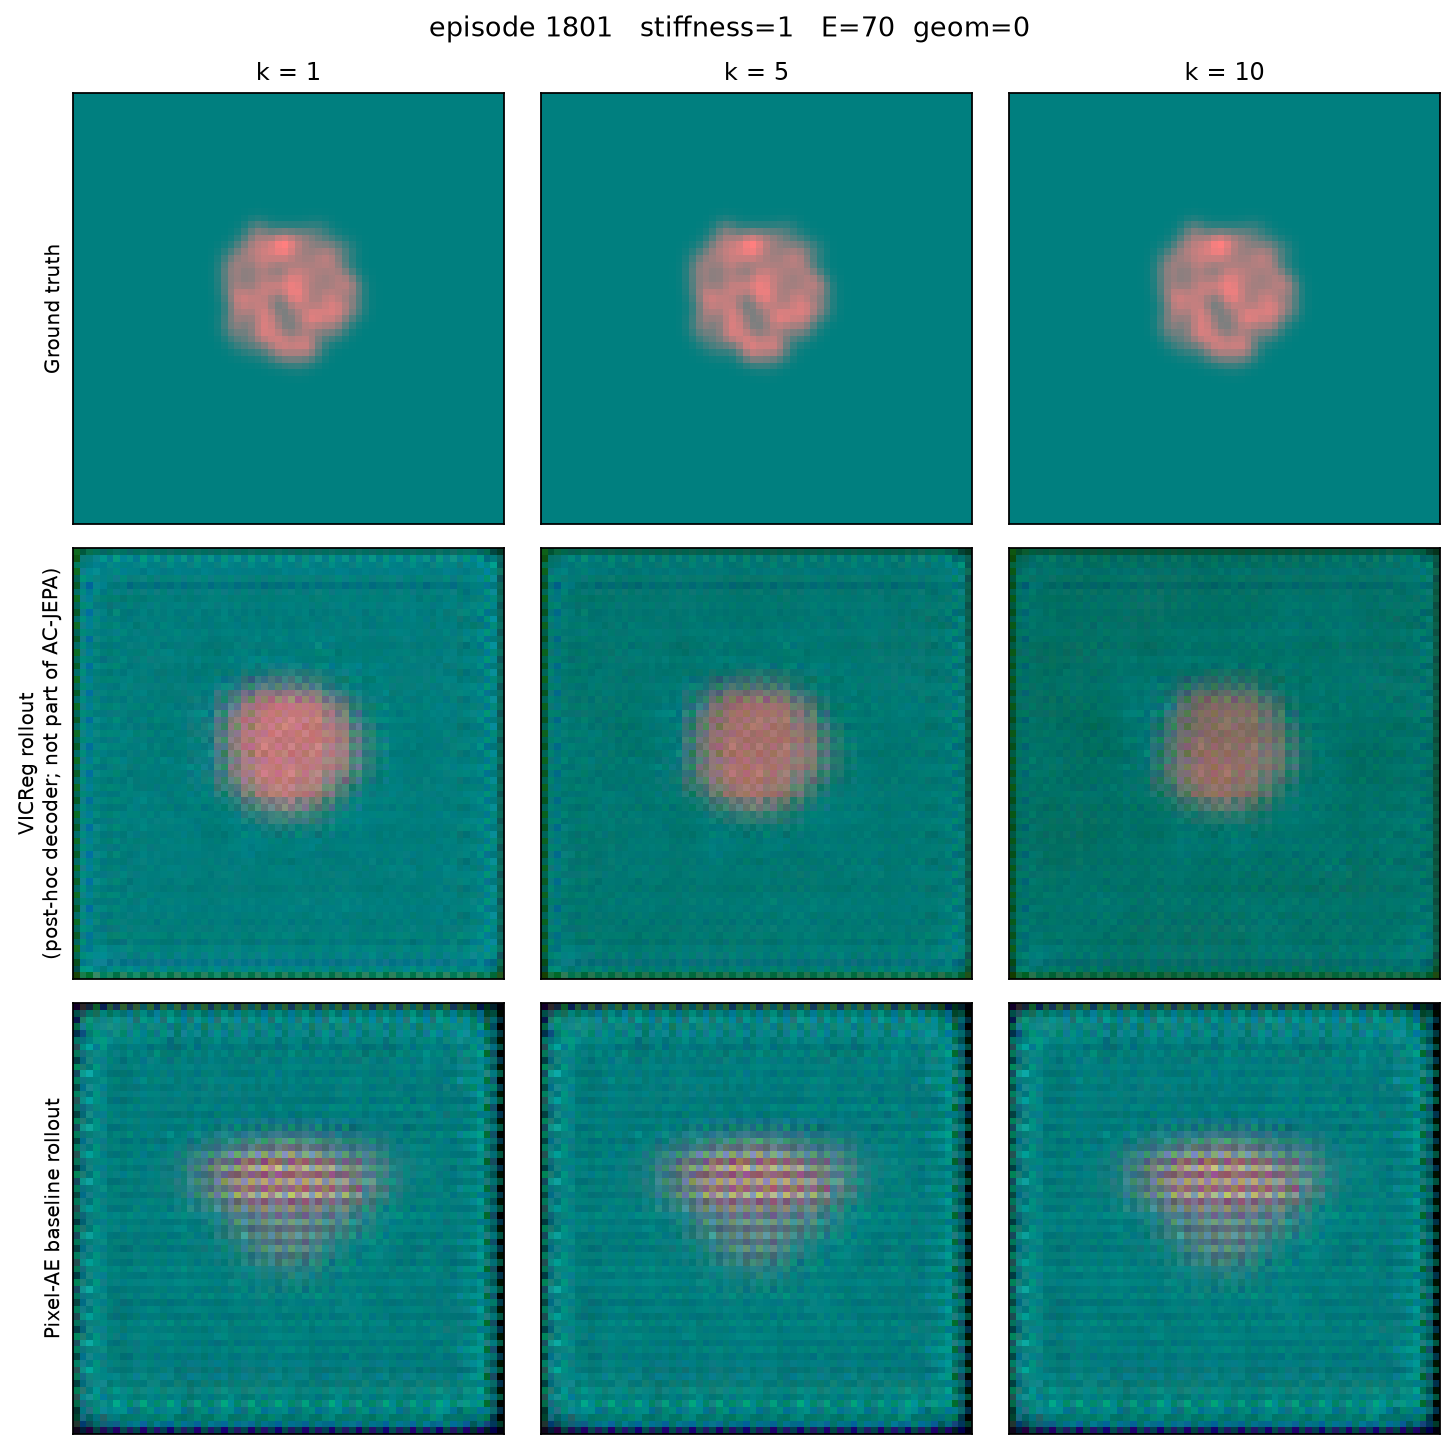
\includegraphics[width=\linewidth]{../outputs/figures/rollout_comparison_1801.png}\\[-2pt]
    {\scriptsize $E{=}\StiffEMid$ (ep.\ \ShowcaseEpB{})}
  \end{minipage}\hfill
  \begin{minipage}{0.32\linewidth}
    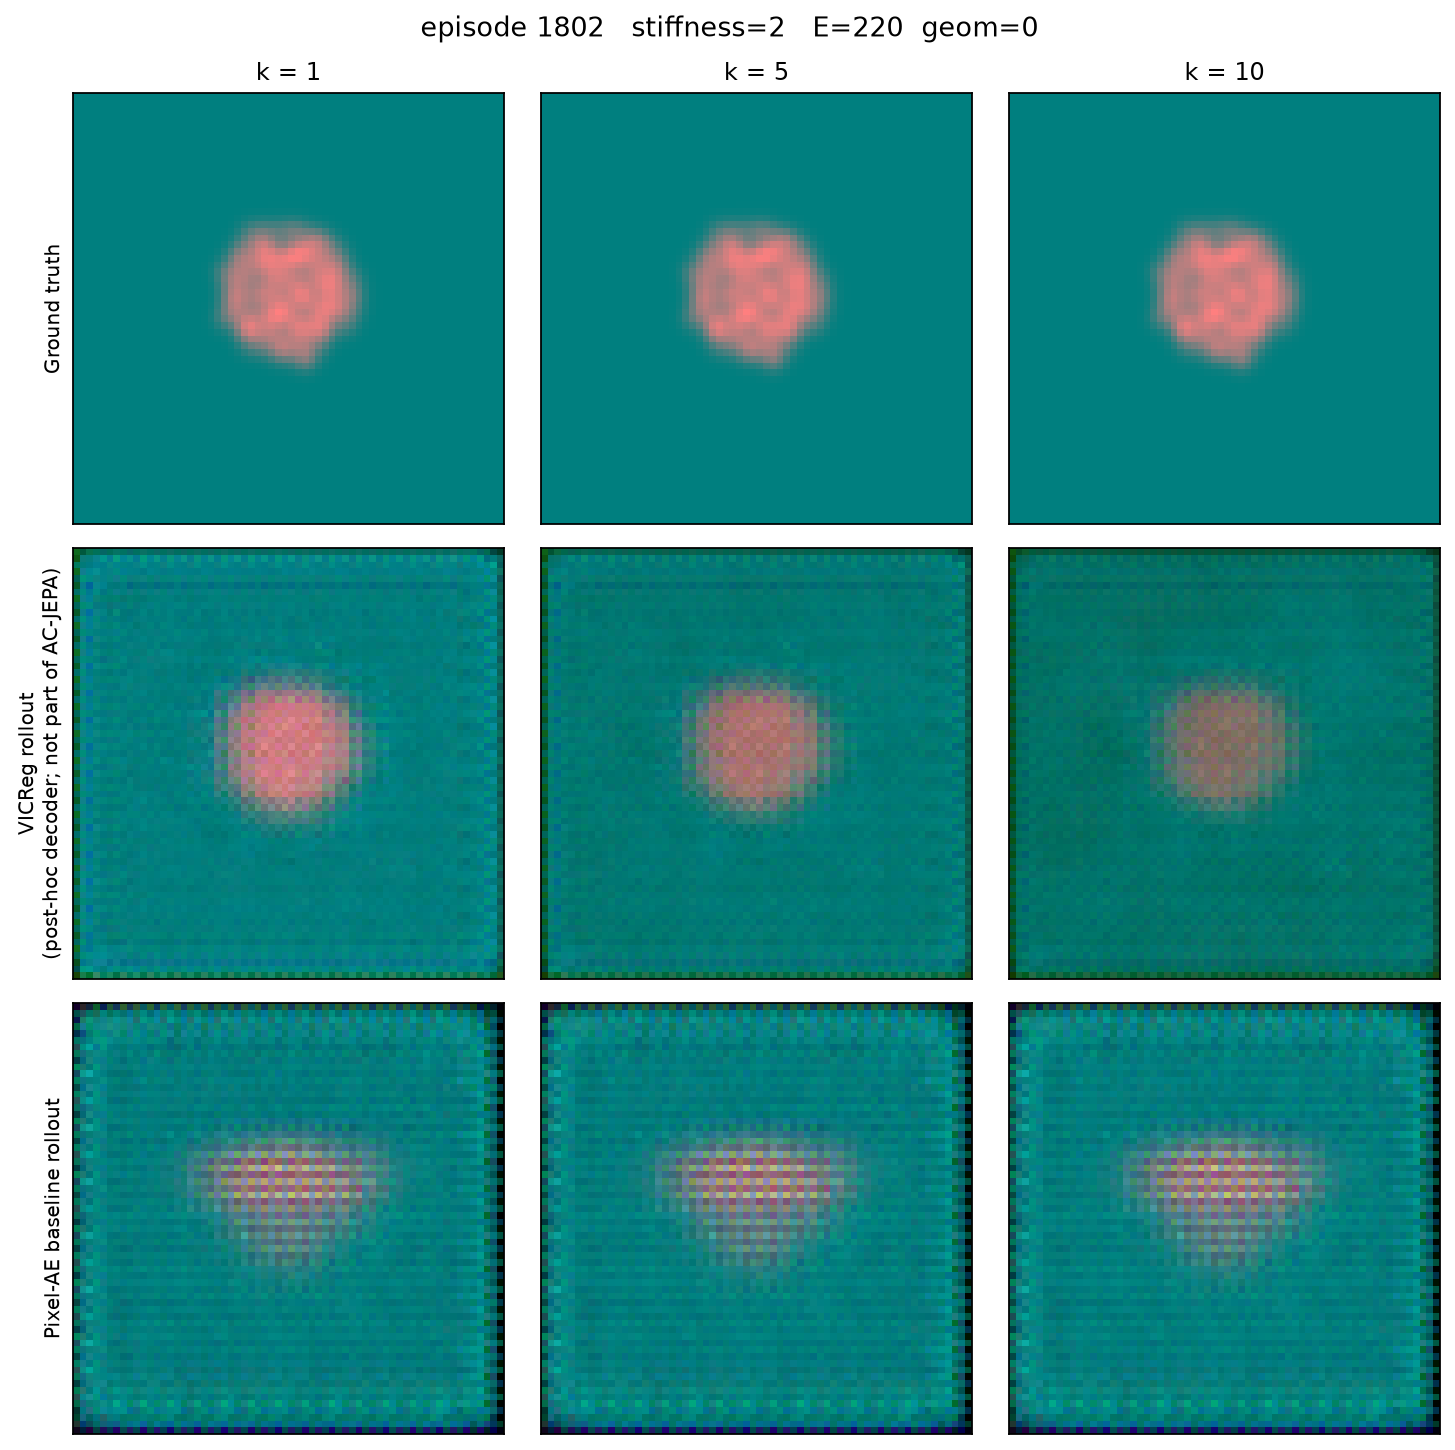
\includegraphics[width=\linewidth]{../outputs/figures/rollout_comparison_1802.png}\\[-2pt]
    {\scriptsize $E{=}\StiffEHigh$ (ep.\ \ShowcaseEpC{})}
  \end{minipage}
  \caption{GT $|$ post-hoc-decoded VICReg $|$ Pixel-AE at $k\in\{1,5,10\}$ on the
  MLS-MPM dump. VICReg weights are an in-progress workshop checkpoint
  (\texttt{outputs/vicreg/best.pt}); Pixel-AE is a short qualitative fit.
  Source: \texttt{outputs/figures/}.}
  \label{fig:rollouts}
\end{figure}

\begin{figure}[t]
  \centering
  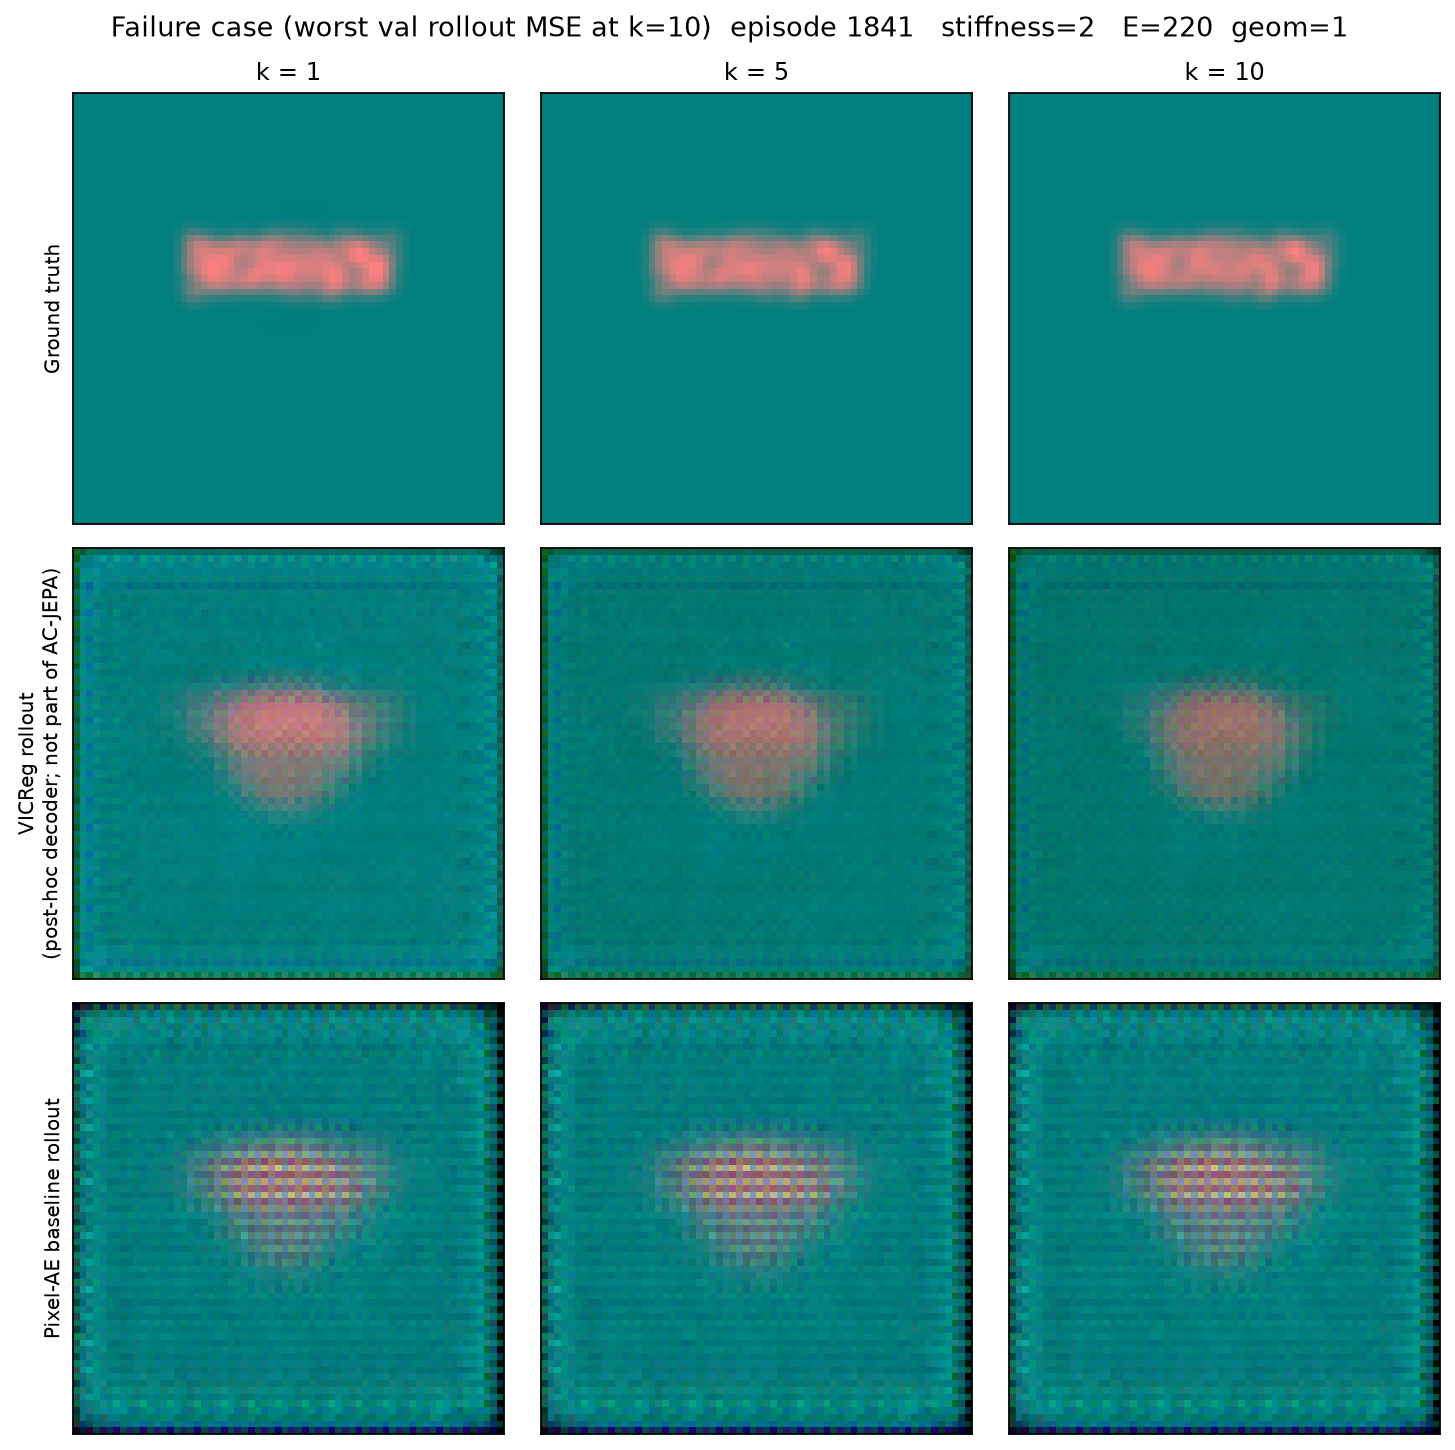
\includegraphics[width=0.62\linewidth]{../outputs/figures/failure_case.png}
  \caption{Episode \FailureEpisode{} ($E{=}\StiffEHigh$), worst val latent MSE at
  $k{=}10$ (\FailureMseKten). Caption text is
  \texttt{outputs/figures/failure\_case\_caption.txt}, grounded in
  \texttt{probe\_diagnostics.json}: stiffness stays at chance, $z_{\mathrm{target}}$
  is collapsed, contact probes beat chance. Not a contact-extrapolation story.}
  \label{fig:failure}
\end{figure}

\section{Limitations}
\label{sec:limitations}
\paragraph{Probes.}
Smoke-split probes in \texttt{outputs/metrics.json} use $n_{\mathrm{val}}{=}$\SmokeNVal{}
and are underpowered (binomial SE $\approx \SmokeProbeSE{}$ at chance \ChanceStiffness{}). On the physics
dump we do have a powered readout. Findings copied from
\texttt{outputs/probe\_diagnostics.json}:

\begin{quote}
\small
Linear-probe findings copied from \texttt{outputs/probe\_diagnostics.json} (\texttt{models.vicreg\_physics\_mpm.findings}):
\begin{itemize}\setlength{\itemsep}{2pt}\setlength{\parsep}{0pt}
    \item stiffness class: after scaling to n\_val=200, mean val acc=0.339 is still consistent with chance=0.333 (z=0.16, SE≈0.033). This is a real limitation: a linear readout of stiffness class from the latents does not beat chance.
    \item contact quadrant: mean val acc=0.574 is above chance=0.250 (z=10.58, n\_val=200).
    \item stiffness class (z\_target): after scaling to n\_val=200, mean val acc=0.331 is still consistent with chance=0.333 (z=-0.08, SE≈0.033). This is a real limitation: a linear readout of stiffness class (z\_target) from the latents does not beat chance.
\end{itemize}
Checkpoint caveat (same file, \texttt{checkpoint\_note}): Copied from outputs/vicreg/best.pt during the in-progress 200-epoch workshop run (not the finished checkpoint).
\end{quote}


Mean stiffness-class val acc is \ProbeStiffValMean{} vs.\ chance
\ChanceStiffness{}; the EMA-target oracle is \ProbeStiffTargetMean{}; train acc
is \ProbeStiffTrainMean{}; Young's-modulus regression $R^2$ averages
\ProbeStiffValRTwo{}. Contact-quadrant val acc is \ProbeContactValMean{} vs.\
chance \ChanceContact{}. $z_{\mathrm{target}}$ occupies a near-constant shell
($\lVert z\rVert$ std \ZTNormStd{}; \ZTDimsBelowGamma{}/\ZTLatentDim{} dims below
the VICReg $\gamma{=}$\VicregGamma{} hinge; hinge binding \texttt{\ZTHingeBinding{}}). We treat
stiffness non-decodability as a limitation of this encoder, not a result to
suppress. The physics VICReg checkpoint is from in-progress workshop training,
not a finished \WorkshopEpochs{}-epoch run.

\paragraph{Domain gap and scale.}
PhysWorld and PhysTwin start from real video and a reconstructed MPM twin. We
render \NEpisodes{} short ($T{=}$\EpisodeLength{}) synthetic clips at
$\ImgSize^2$ with \NStiffClasses{} discrete global $E$ values. That is orders of magnitude
away from real-video digital-twin benchmarks in appearance, geometry, and
parameter identification. Nothing here should be quoted as evidence on those
benchmarks.

\paragraph{Missing scaled ablations.}
The planned multi-seed workshop grid that would populate Table~\ref{tab:ac-jepa-ablation-multiseed}
has not been written. Table~\ref{tab:ac-jepa-ablation} is dummy-scale.
\texttt{outputs/ablation\_drift.png} was overwritten by a different smoke run and
is not used. Git HEAD does not contain the code that produced these artifacts
(\texttt{MAPPING.md}).

\section{Conclusion}
AC-JEPA on synthetic deformables is a setting in which action conditioning
changes latent rollout error on a shared mass-spring split, VICReg's extra
terms do not automatically win latent MSE against a pure invariance baseline,
and a scaled linear probe can read contact quadrant but not stiffness. Those
are the claims this repository currently supports. They are not a SOTA result
on real video.

\bibliography{references}
\bibliographystyle{plainnat}

\end{document}
